\title{Supplements}

\documentclass[12pt]{article}
\usepackage{amsmath}
\usepackage{mathabx}
\usepackage{graphics}
\usepackage[top=0.5in, bottom=0.5in, left=1in, right=1in]{geometry}
\usepackage{tabu}
\usepackage[english]{babel}
\usepackage{natbib}
\bibliographystyle{evolution}
\usepackage{rotating}
\usepackage[capitalize, sort&compress]{cleveref}
\usepackage{float}
%\newcommand{\crefrangeconjunction}{--}
%\crefname{section}{Sect.}{Sects.}
%\crefname{equation}{Eq.}{Eqs.}
%\crefformat{equation}{Eq.~#2#1#3}
%\crefrangeformat{equation}{Eqs.~#3#1#4--#5#2#6}
%\crefmultiformat{equation}{Eqs.~#2#1#3}{--#2#1#3}{, #2#1#3}{ and~#2#1#3}
 
% for comments visible in the compiled pdf
%\usepackage{color}
%\definecolor{orange}{rgb}{0.8,0.4,0}
%\newcommand{\eeg}[1]{{\em \color{orange} #1}}

% Tell latex how it can introduce linebreaks if necessary.
\hyphenation{Bar-thol-o-mew}

\date{\vspace{-5ex}}

\begin{document}
\maketitle 

The supplementary file contains supplementary text and figures for sensitivity analyzes with respect to Fig. 2def, Fig. 4, and Fig. 6 from the main manuscript.
Figure S1  shows the results for different coefficient and exponent for the active metabolic  rates  when resources are unlimited (Fig.~S\ref{figS1}). 
The first row shows that when to cost of active metabolic rate is low, temperature, exponent of foraging rate $b_3$, large is always advantageous.
The second row shows the effect of the coefficient $a_2$ while keeping $b_2 = b_1 = 0.75$, the cost can be so high at high temperature that net energy gain is always negative.
Otherwise, small is never favored.
The third row shows the effect of the exponent $b_2 = 1.25$ while keeping $a_2 low$.
Only when $b_3$ is highly concave and temperature is high that intermediate body size becomes advantageous.

Figure S2  upper row shows the minimum temperature for completing warm-up when operative temperature is independent of body mass  (i.e., $c_1 = 0$) (Fig.~S\ref{figS2}).
When operative temperature $T_w$ is independent of body size, warm-up ability always increases or decreases as function of body size.
Figure S2 lower row shows the minimum temperature for completing warm-up when more solar radiation is absorbed (i.e., $r_3 = 0.75$) (Fig.~S\ref{figS2}).
It shows that under without wind and low convection factor (dashed lines) and with sufficient solar radiation any body size can complete warm-up.

Figure S3 shows the effect of relaxing constant temperature for the duration of warm-up (Fig.~S\ref{figS3}).
At sunrise, the environmental temperature is  $15 ^{\circ}\rm{C}$ at sunrise (around 6 a.m.) and rises linearly until the middle of the afternoon (around 3 p.m.) to reach $30 ^{\circ}\rm{C}$.
Figure S3 shows that adding changes in environmental temperature does not changes the qualitative results (see Fig. 5 in the main text).
Figure S3 also shows that duration of warm-up increases with body size expect when the individual is too small and warm-up starts early.

Figure S4 shows the effect of relaxing constant temperature (Fig.~S\ref{figS4}).
The x-axis shows the initial temperature at sunrise (coldest) then increases linearly until it peaks at the middle of the afternoon (midpoint between noon and sunset). The hottest temperature is defined by an increase of $10 ^{\circ}\rm{C}$ (left panels) or $20 ^{\circ}\rm{C}$ (right panels) from the temperature at sunrise.
Figure S4 shows that adding changes in environmental temperature does not changes the qualitative results (see Fig. 6 in the main text).

For all the figures, the remaining parameters are the same as in the main text.

\begin{figure*}
%\begin{center}
	\scalebox{0.85}{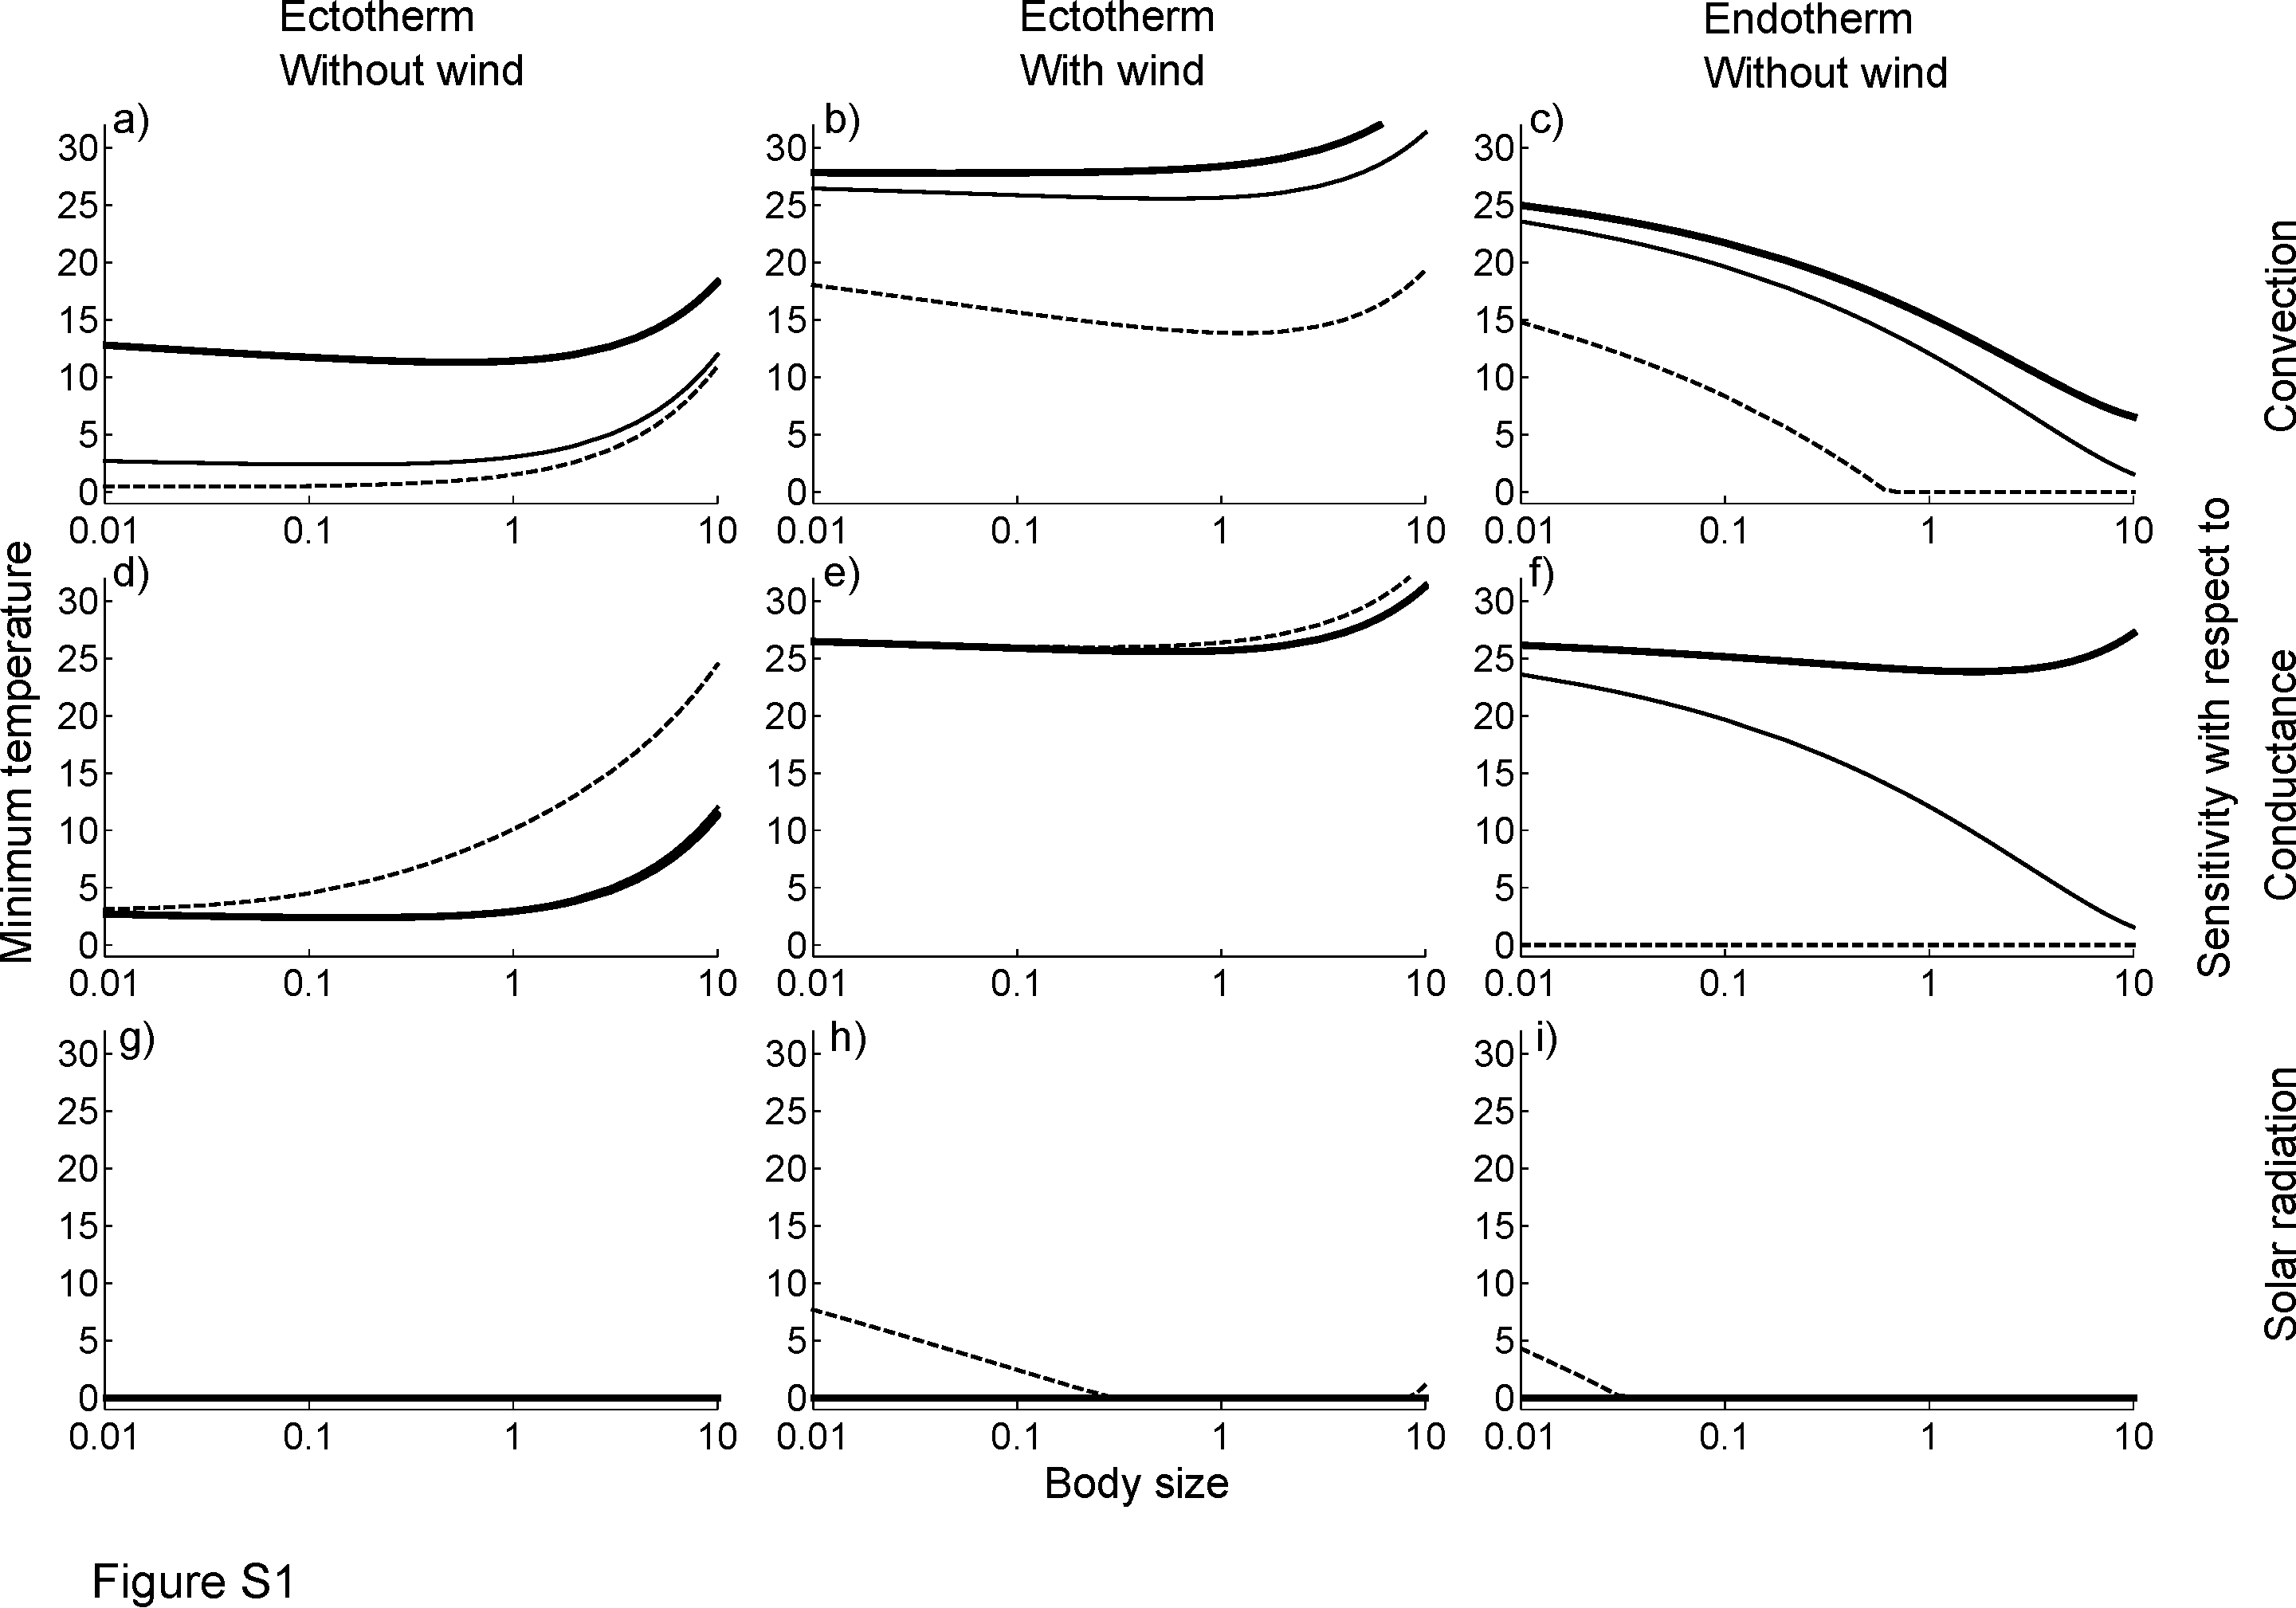
\includegraphics{figS1}}
	%\caption{Figure S1}
	\label{figS1}
%\end{center}
\end{figure*}


\begin{figure}
%\begin{center}
	\scalebox{0.75}{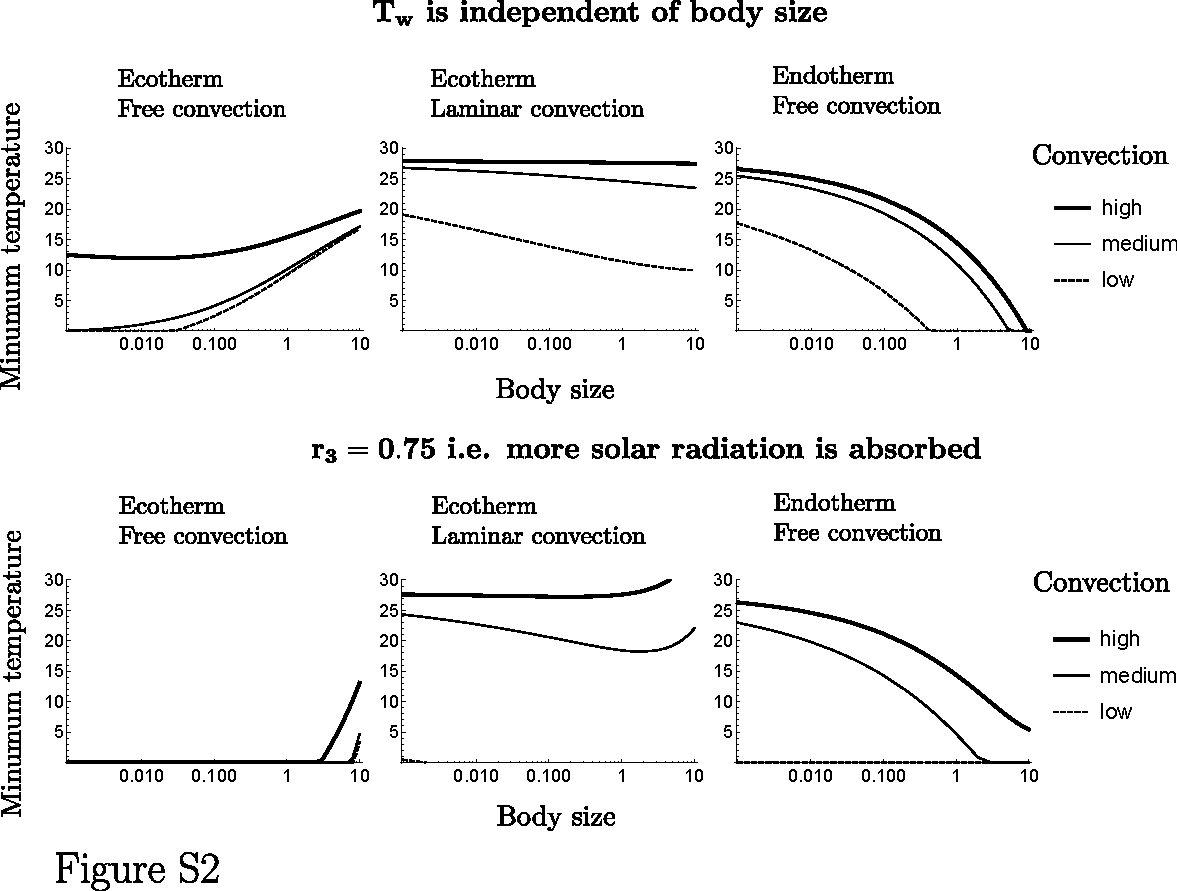
\includegraphics{figS2}}
	%\caption{Figure S2}
	\label{figS2}
%\end{center}
\end{figure}

\begin{figure}
%\begin{center}
	\scalebox{0.75}{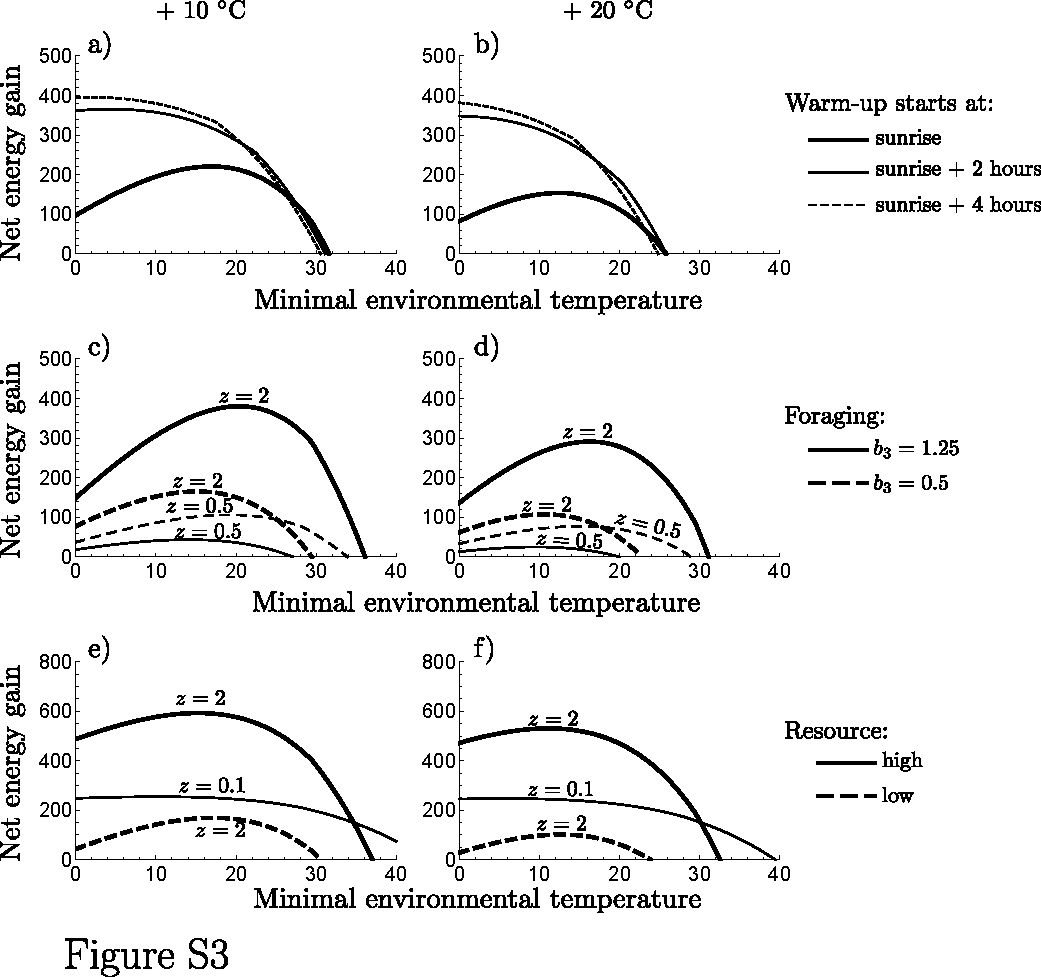
\includegraphics{figS3}}
	%\caption{Figure S2}
	\label{figS2}
%\end{center}
\end{figure}

\begin{figure}
%\begin{center}
	\scalebox{0.85}{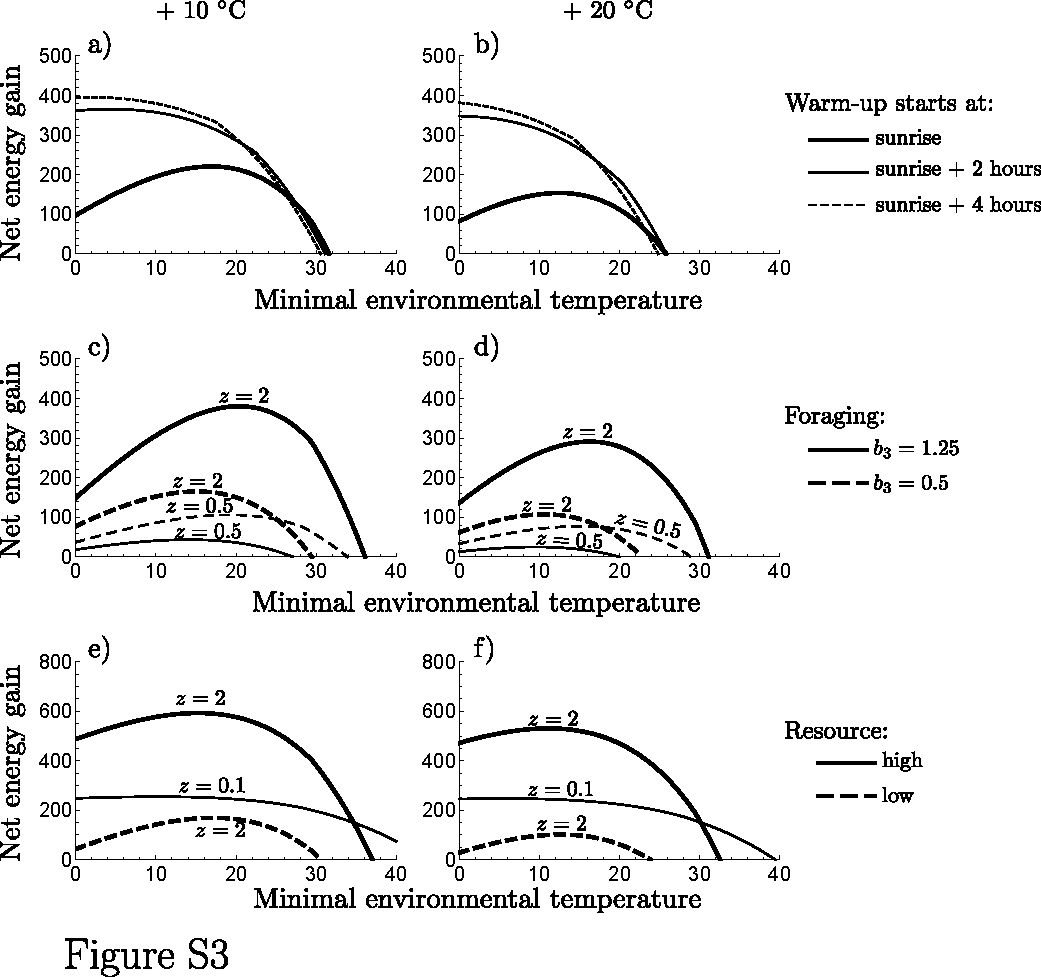
\includegraphics{figS4}}
	%\caption{Figure S3}
	\label{figS3}
%\end{center}
\end{figure}

\end{document}
